\documentclass[letterpaper,12pt]{article}

\usepackage{graphicx}


\author{Daniel Ricard}
\title{Details about the stock-recruitment database design, configuration and operation}


\begin{document}
\maketitle

\section{Database server configuration}

The stock-recruitment database is created on the postgresql server and is owned by the ``srdbadmin'' user. To achieve this, the database server owner (usually, the postgres user) needs to create a SUPERUSER database role called ``srdbadmin'':
\begin{verbatim}
CREATE ROLE srdbadmin WITH SUPERUSER;
\end{verbatim}

Next, the database server owner creates a new database called ``srdb'' which is owned by ``srdbadmin'':
\begin{verbatim}
sudo -u postgres createdb srdb -O srdbadmin  
\end{verbatim}

The empty ``srdb'' database is now owned by ``srdbadmin''. The next tasks are to 1) create the database tables, 2) populate the database with data and 3) configure the database with correct access permissions for the different users that will be using it.

To achieve an acceptable level of access to the stock-recruitment database while maintaining database intergity and security, the database server must be configured appropriately and access rules to the database must be specified. The basic idea behind the database configuration is that the database user called ``srdbadmin'' is the owner of all database tables and views, and has all privileges on the database. This means that this user can CREATE, DROP, MODIFY, INSERT, etc. In comparison, another database user called ``srdbuser'' only has the ability to SELECT data from the database and can't damage its integrity.

Additionally, to handle different research projects that use the database, a few other database users are created based on the project name. These users have SELECT permissions on all database tables and also have the ability to CREATE tables in their own schema. This is deemed useful for writing database tables of model fit results, for example, without cluttering the ``srdb'' schema which is used for the stock-recruitment database tables.

The database users are created using ``CREATE ROLE'' while logged in as the database server administrator. 

\begin{verbatim}

 
\end{verbatim}


All database tables are contained within the ``srdb'' schema and the privileges to access them must be granted by the database owner. In postgreSQL this is best done by a little script that specifies the proper permissions to the different users. In our case, the owner of the database will GRANT SELECT to ``srdbuser'' for all tables in the ``srdb'' schema.

In terms of database server configuration, there are two files of interest:

\begin{description}
 \item [pg\_ident.conf]{identification configuration file}
 \item [pg\_hba.conf]{host-based authentication configuration file}
 \end{description}



\section{Database design}

The database design is inspired by RAM's original work. The stock-recruitment database consists of a variety of tables related to each other through primary and foreign keys. 


The Entity Relationship Diagram shown in Figure~\ref{fig:erd} shows the different tablea and their relationships to each other.

\begin{figure}
 \begin{center}
 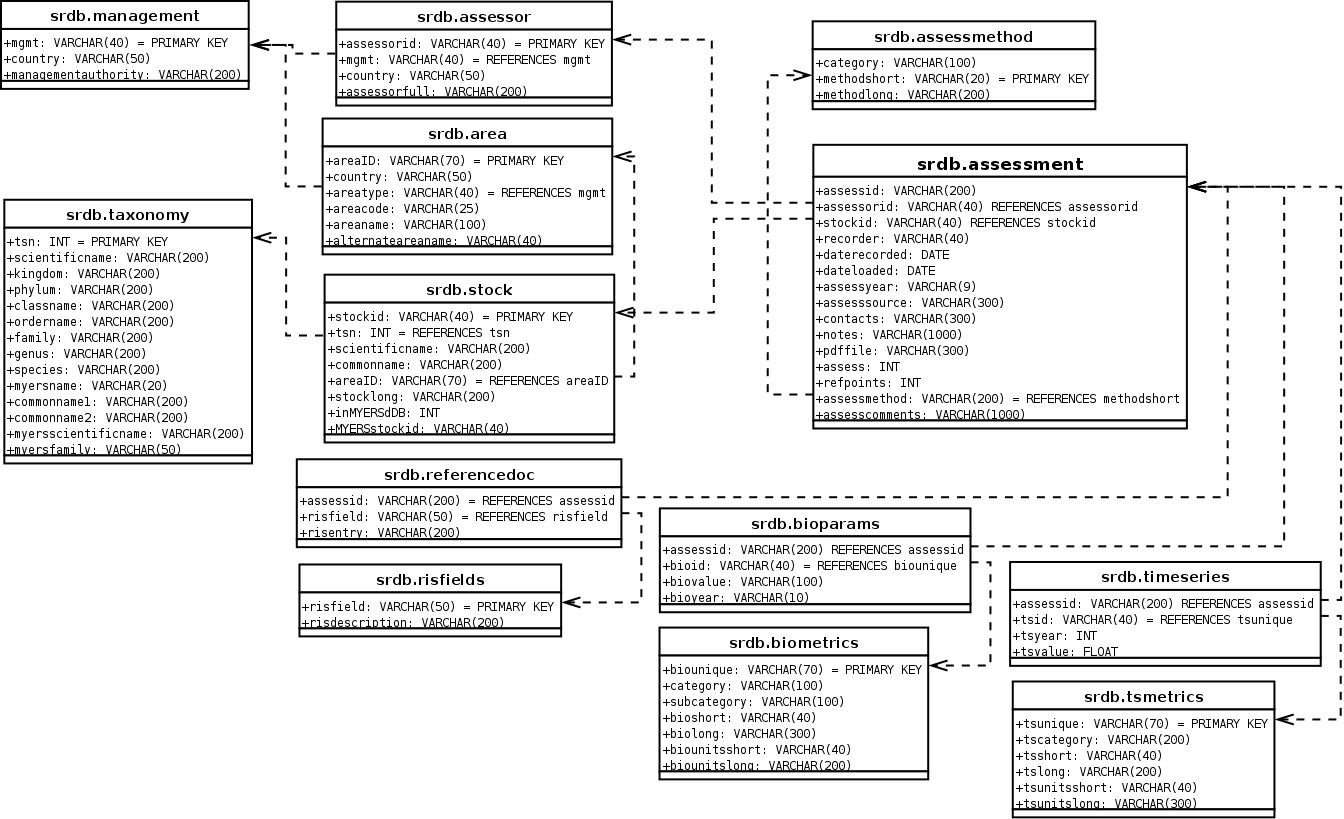
\includegraphics[angle=90, scale=0.3] {srdb-ERD.png}
 % srdb-ERD.png: 1267x785 pixel, 51dpi, 63.35x39.25 cm, bb=0 0 1796 1113
\end{center}

\caption{Entity relationship diagram of the stock-recruitment database.}\label{fig:erd}
\end{figure} 


Each assessment that is loaded in the databse is added to the srdb.assessment table and the data itself is added to the srdb.timeseries and srdb.bioparams tables.


\section{Database scripts}


The stock-recruitment database is created, populated and optimized through a series of shell scripts. 

Table definitions are invoked first. The background data is then loaded in the database. The assessment spreadsheets are loaded next. Indices, views and other bookkeeping tools are finally activated.


To reduce the number of units in the time-series data, all biomass and abundance time-series are modify so that data is vailable in metric tonnes (MT) for biomass and in thousands (E03) for abundance. 


\section{Database quality-control}



\section{Database views for different projects and clients}



\end{document}
